\documentclass[UTF8,a4paper]{ctexart}
\usepackage{graphicx}
\usepackage{geometry}
\geometry{a4paper,scale=0.8}
\usepackage{setspace}
\setstretch{1.6}

\begin{document}
\begin{sloppypar}
	
	\begin{center}
		\begin{fontsize}{80pt}{20pt}
			实验报告
		\end{fontsize}

		\bigskip
		\bigskip
		
		\begin{fontsize}{35pt}{20pt}
			\begin{flushright}
				—— {\Huge Git}与{\Huge Latex}的学习与使用
			\end{flushright}
		\end{fontsize}
		
		\bigskip
		\bigskip
		\bigskip
		\bigskip
		\bigskip
		\bigskip
		\bigskip
		\bigskip
		\bigskip
		\bigskip
		\bigskip
		\bigskip
		\bigskip
		\bigskip
		\bigskip
		\bigskip
		
		\begin{fontsize}{25pt}{20pt}
			姓名:
			\underline{翟一航}
			
			\bigskip
			\bigskip
			\bigskip
			\bigskip
			
			学号:
			\underline{{\huge 23020011046}}
			
			\bigskip
			\bigskip
			\bigskip
			\bigskip
			
			班级:
			\underline{{\Huge 23}级软件工程五八班}
			
			
		\end{fontsize}
	\end{center}
	\section{实验要求}
	\subsection{学习版本控制Git的使用}
	\subsection{完成4个课堂练习与20个与Git和Latex有关的实例}
	\subsection{学习用Latex进行文档编辑,并设计自己的实验报告模板}
	\section{实验内容}
	\subsection{Git(Bash)的学习}
	\subsubsection{版本控制系统 (VCSs) 是一类用于追踪源代码(或其他文件、文件夹)改动的工具。顾名思义,这些工具可以帮助我们管理代码的修改历史;不仅如此,它还可以让协作编码变得更方便。VCS 通过一系列的快照将某个文件夹及其内容保存了起来,每个快照都包含了文件或文件夹的完整状态。同时它还维护了快照创建者的信息以及每个快照的相关信息等等。}
	\subsubsection{Git包含以下特点:\\1.分布式存储\\2.数据完整性\\3.分支管理\\4.非线性开发\\5.安全性\\6.轻量级操作\\7.强大的合并和冲突解决功能}
	\subsubsection{Git的基本工作流程通常包括以下几个步骤:\\1.克隆(Clone)\\2.修改(Modify)\\3.提交(Commit)\\4.推送(Push)\\5.拉取(Pull)\\接下来也将围绕这些操作来完成课堂任务与实例应用}
	\subsection{Latex的学习}
	\subsubsection{Latex是一个基于TeX的排版系统,广泛用于生成科学和数学文档。它特别适合于生成包含复杂公式、表格和参考文献的文档。}
	\subsubsection{为了更好地学习与使用Latex来进行文档的编写,我首先根据教程在电脑上安装了Latex Live,配置了Latex的使用环境,接着下载了专门用于撰写Latex文档的工具Texstudio。}
	\subsubsection{通过在网上查阅资料、浏览教学视频,我学会了Latex的一些基本用法,如:设置文档的标题以及文段的格式、插入图片与数学公式、加入拓展的宏和包等,并将这些内容应用在了此次实验报告撰写中。}
	\subsection{课堂练习}
	\subsubsection{克隆课程网站的GitHub仓库,将版本历史可视化并进行探索}
	
	
	克隆课程网站的GitHub仓库,将版本历史可视化并进行探索
	
	首先,在文件资源管理器中找到合适的位置创建一个文件夹,来储存克隆下来的仓库,在Git中先通过cd指令进入相应磁盘中的文件夹。
	
	然后,打开GitHub仓库,复制仓库的链接(如下图所示)
	
	\graphicspath{{figure/}}
	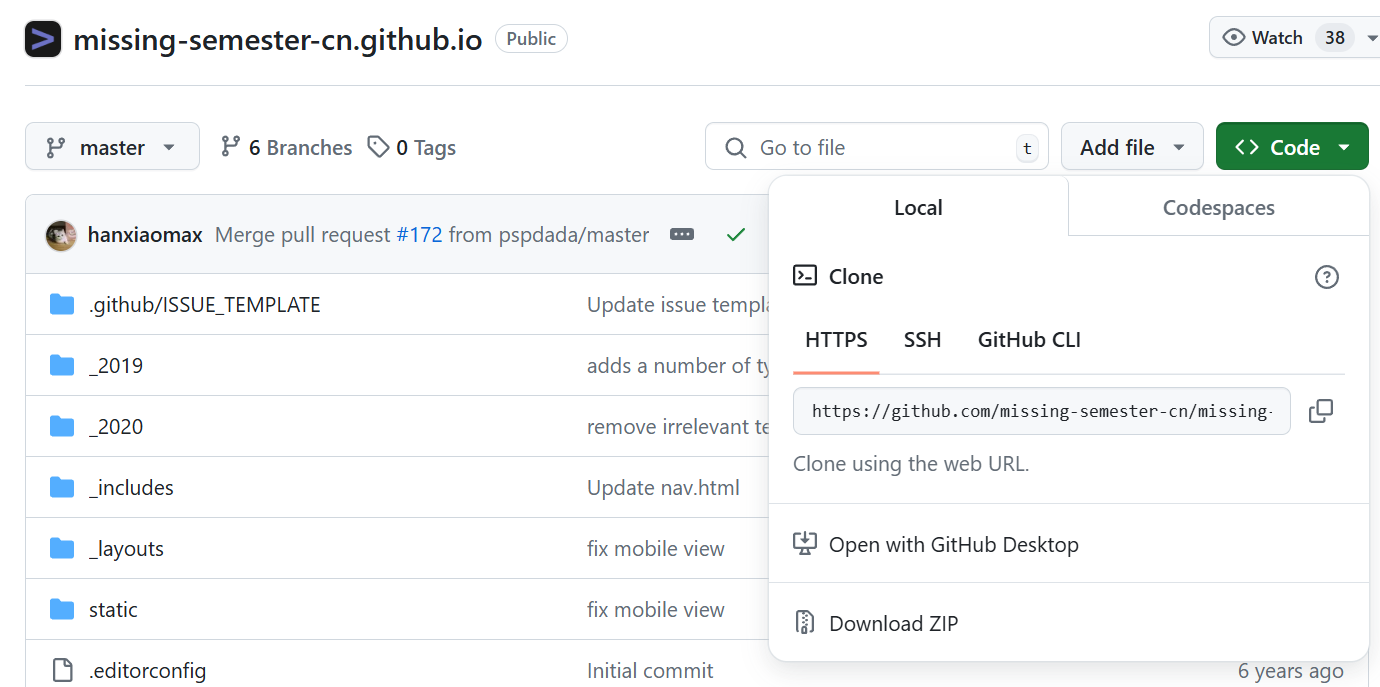
\includegraphics[width = 8cm]{1}
	
	之后,在Git中输入指令git clone https://github.com/missing-semester-cn/missing-semester-cn.github.io.git(链接为刚刚复制而来),接着就会进行仓库的克隆,会显示克隆进度
	
	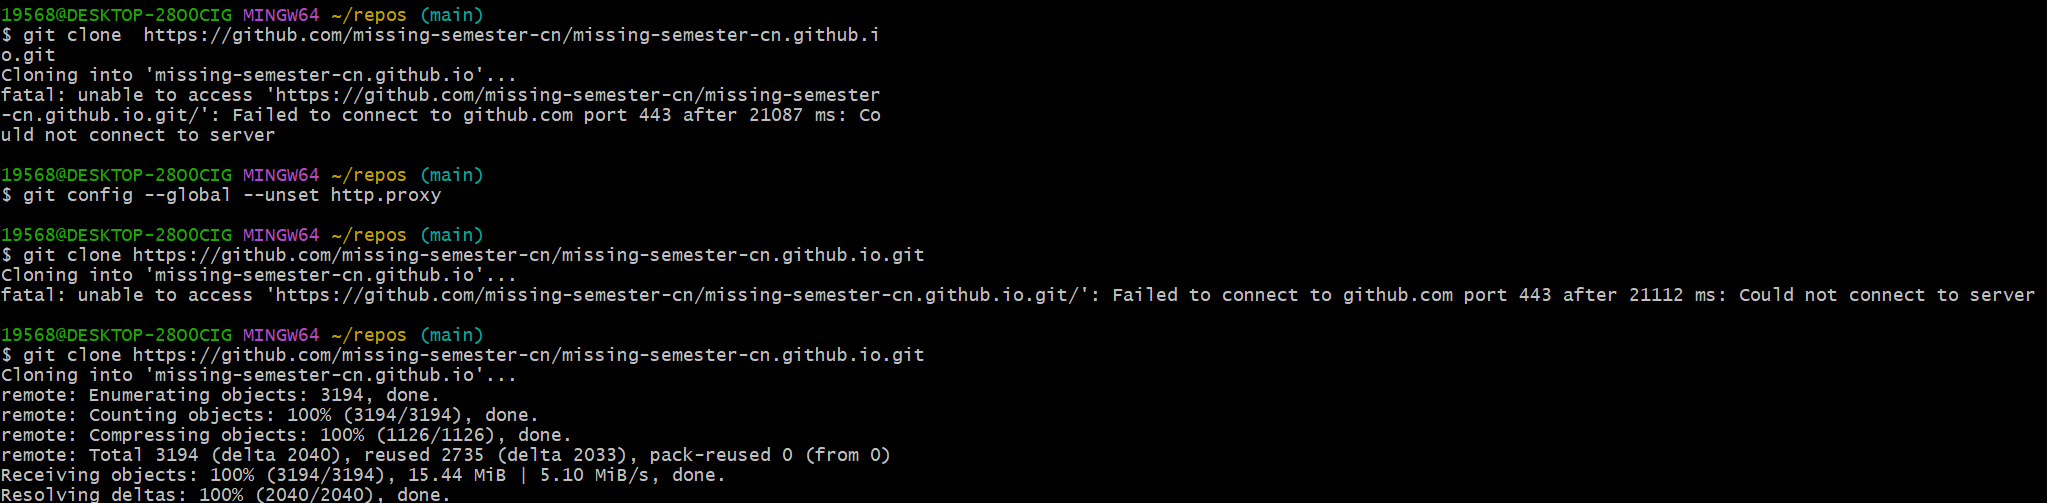
\includegraphics[width = 16cm]{2}
	
	最后,该进行版本历史可视化的探索。在Git中输入指令git log --all --graph --decorate,会出现如下界面,版本可视化探索完成。
	
	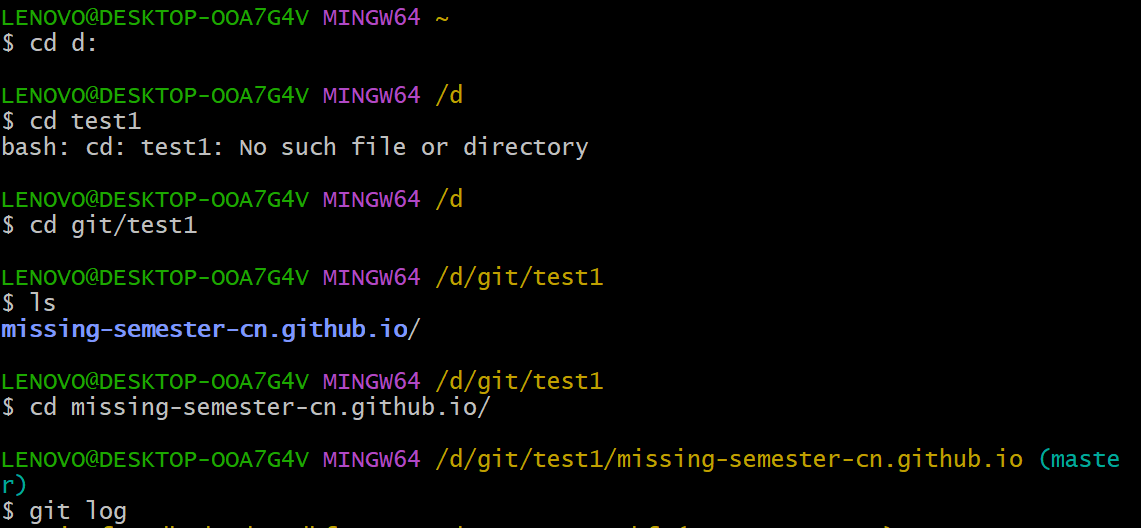
\includegraphics[width = 16cm]{3}
	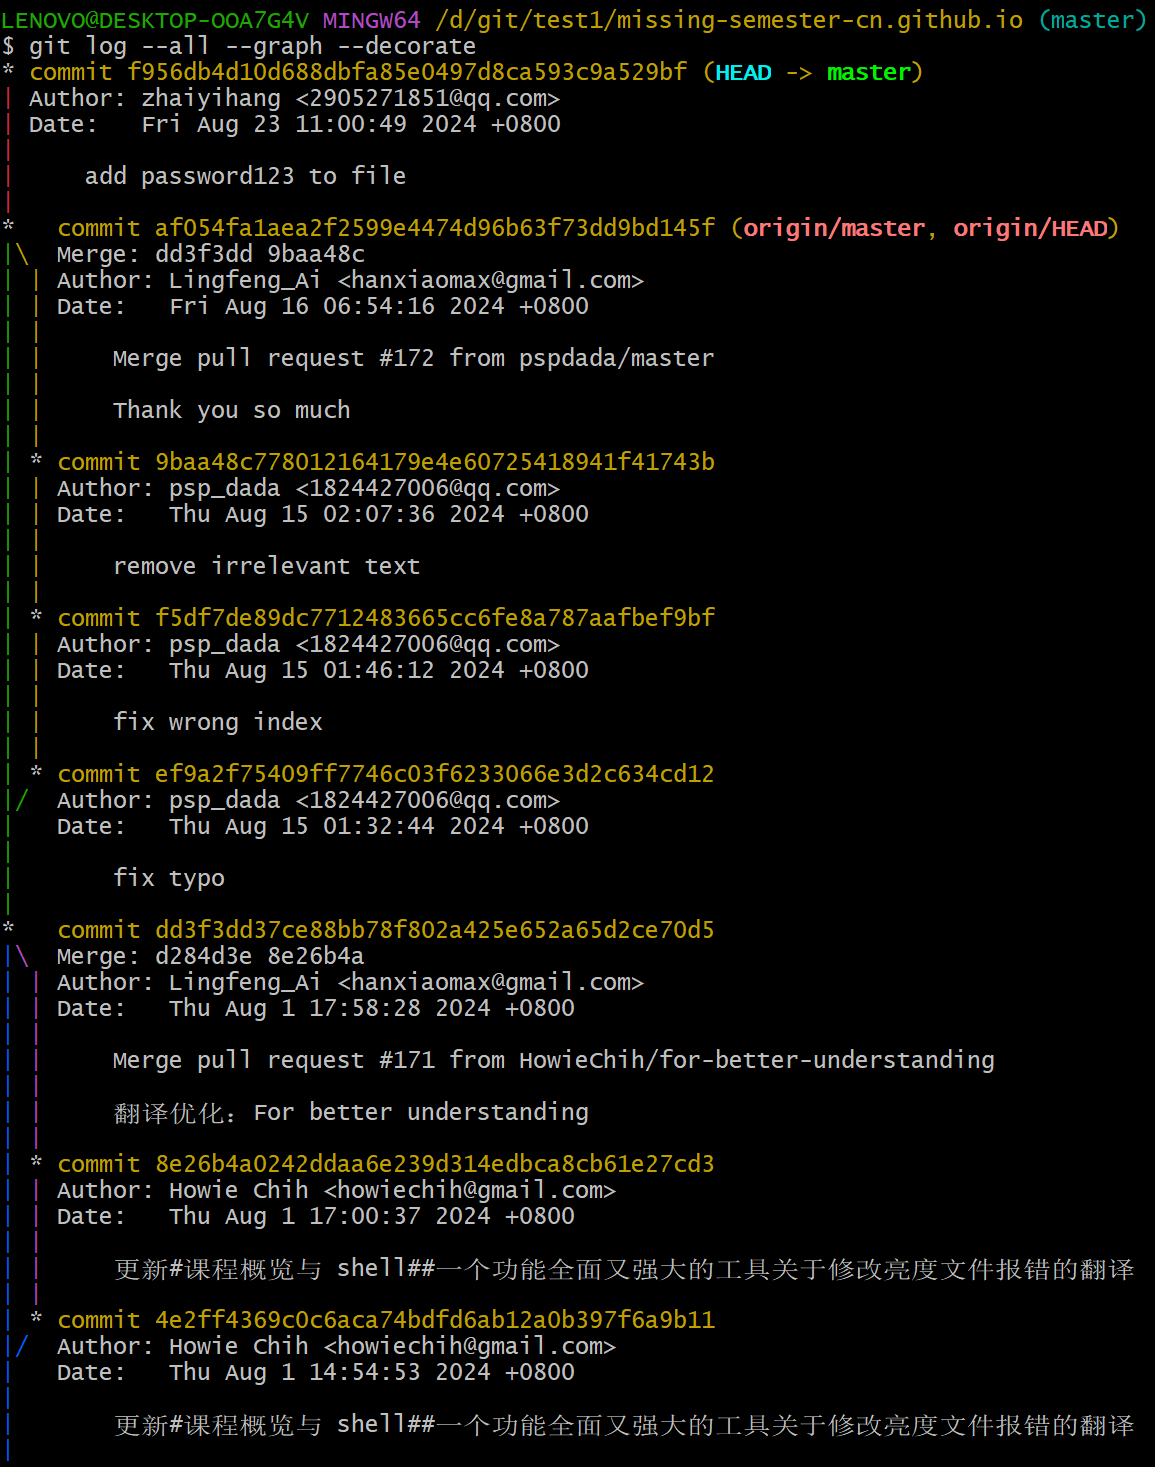
\includegraphics[width = 16cm]{4}
	
	\subsubsection{查看是谁最后修改了 README.md 文件}
	在Git中输入指令git log -1 README.md,其中,-1表示查看最新的 1 次提交或特定文件的版本信息(结果如下图所示)。
	
	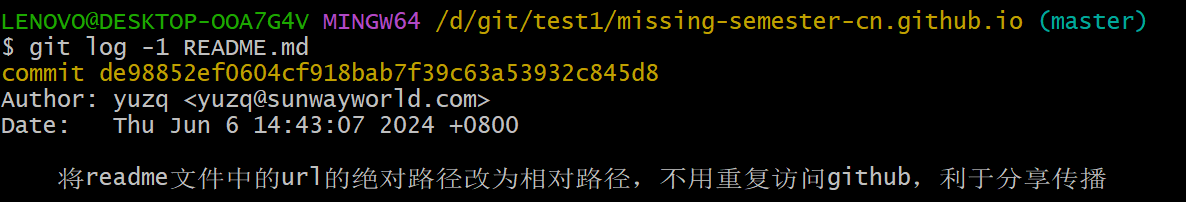
\includegraphics[width = 16cm]{5}
	
	\subsubsection{查看最后一次修改 \_config.yml 文件中 collections: 行时的提交信息是什么}
	在Git中依次输入指令:git blame \_config.yml | grep collections、git show --pretty=format:"\%s" a88b4eac | head -1 出现以下界面即为查看成功。
	
	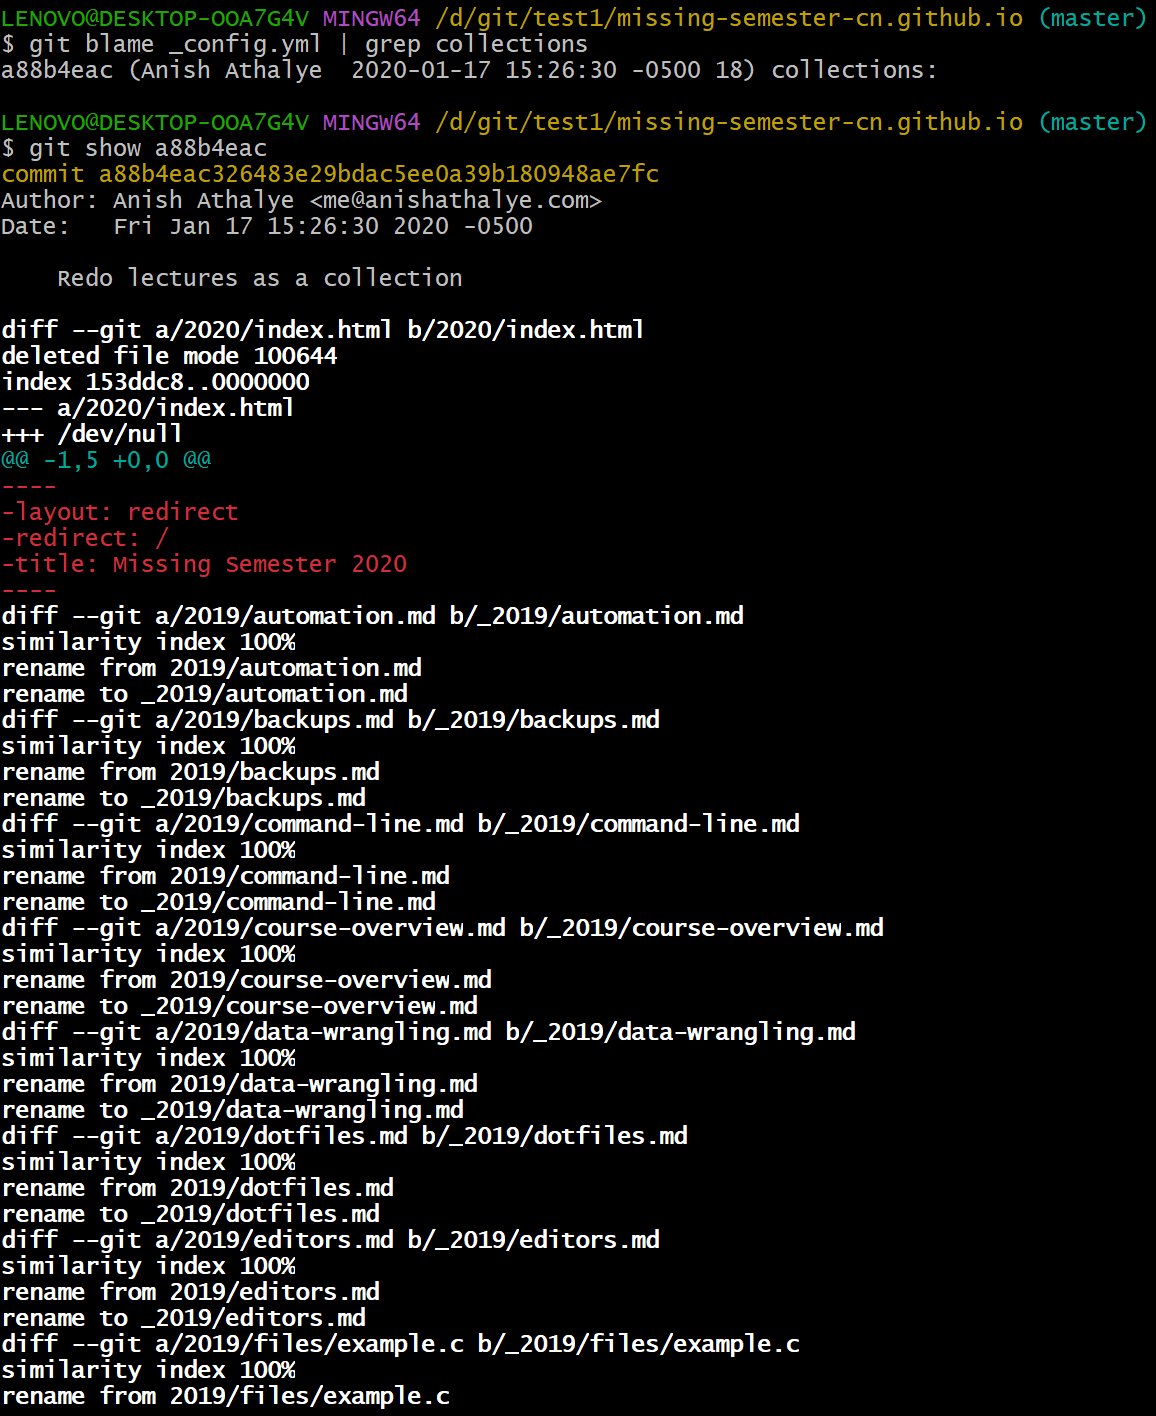
\includegraphics[width = 16cm]{6}
	
	\subsubsection{使用 Git 时的一个常见错误是提交本不应该由 Git 管理的大文件,或是将含有敏感信息的文件提交给 Git 。尝试向仓库中添加一个文件并添加提交信息,然后将其从历史中删除}
	
	首先,我们来提交一些敏感信息,在Git中依次输入echo "password123">my\_password、git add、git commit -m "add password123 to file"、git log HEAD,即可向库中提交密码这一敏感信息。
	
	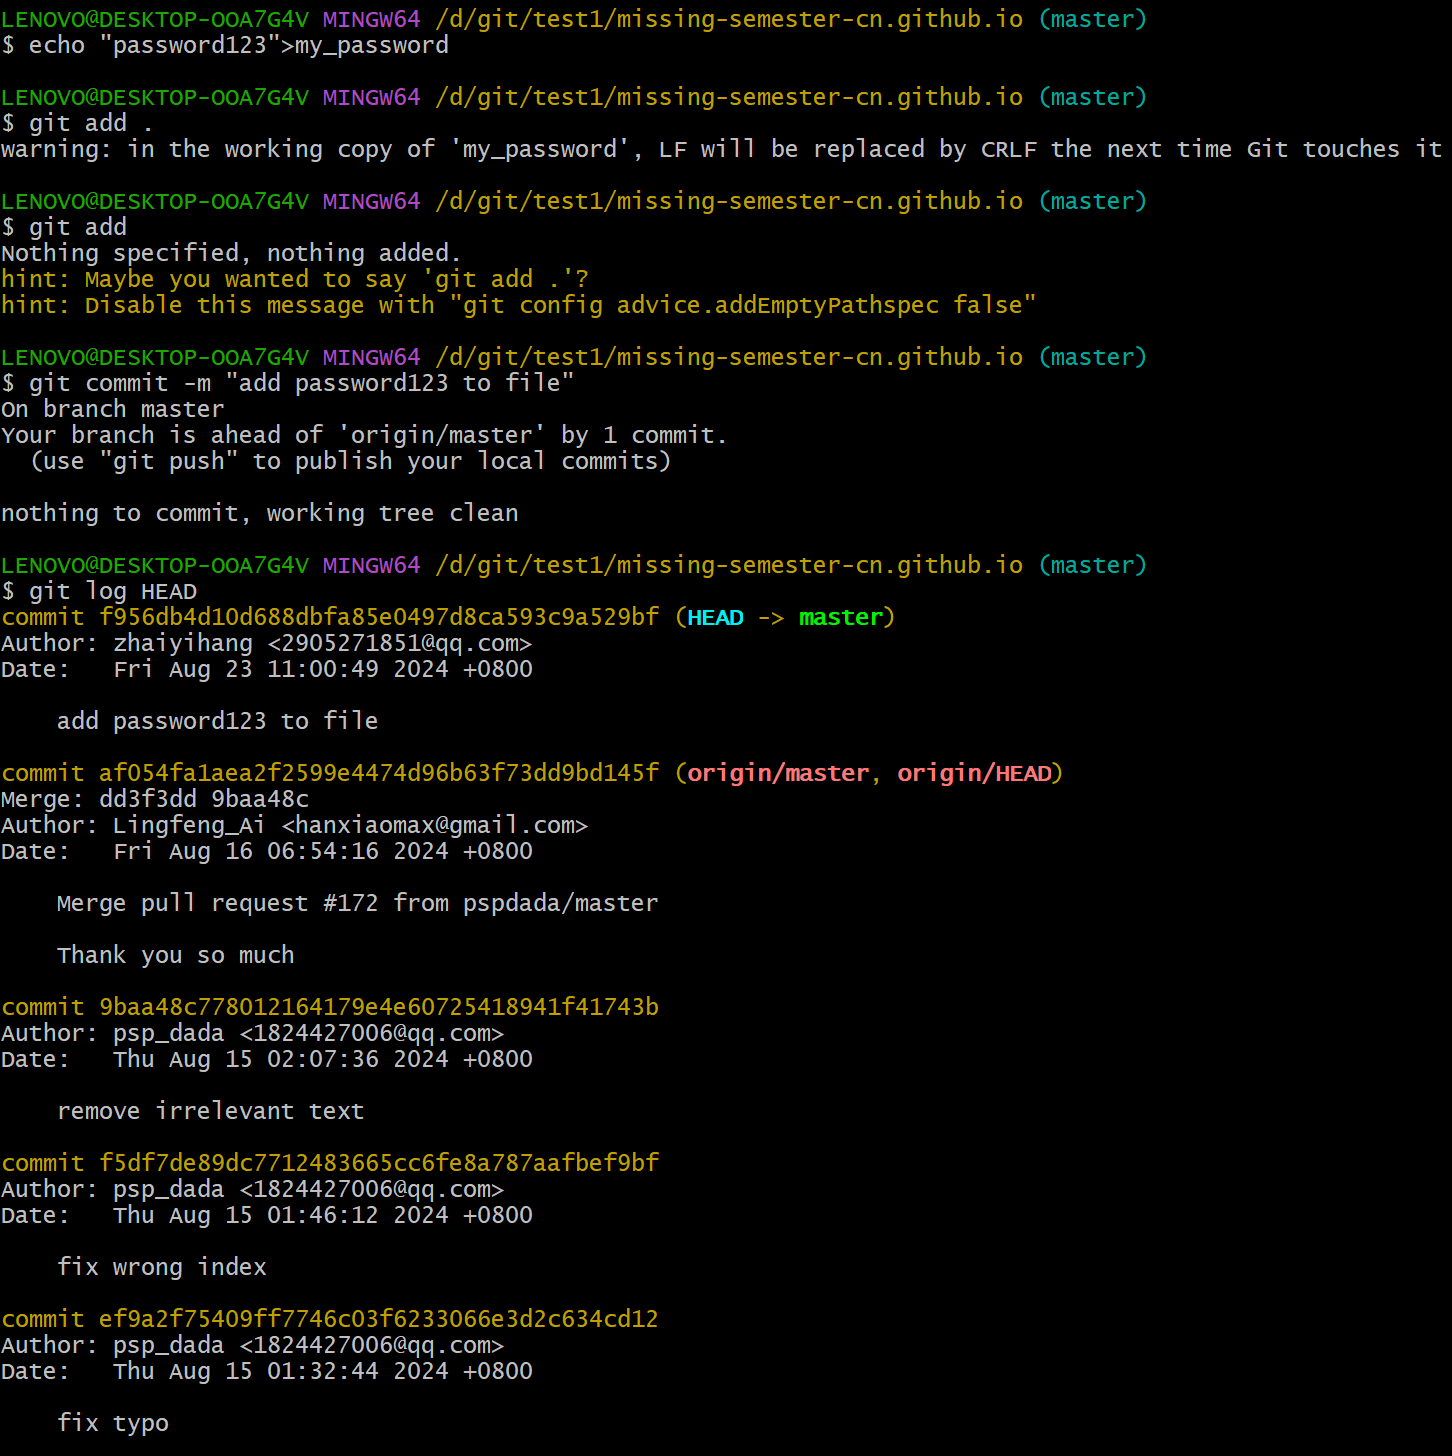
\includegraphics[width = 16cm]{7}
	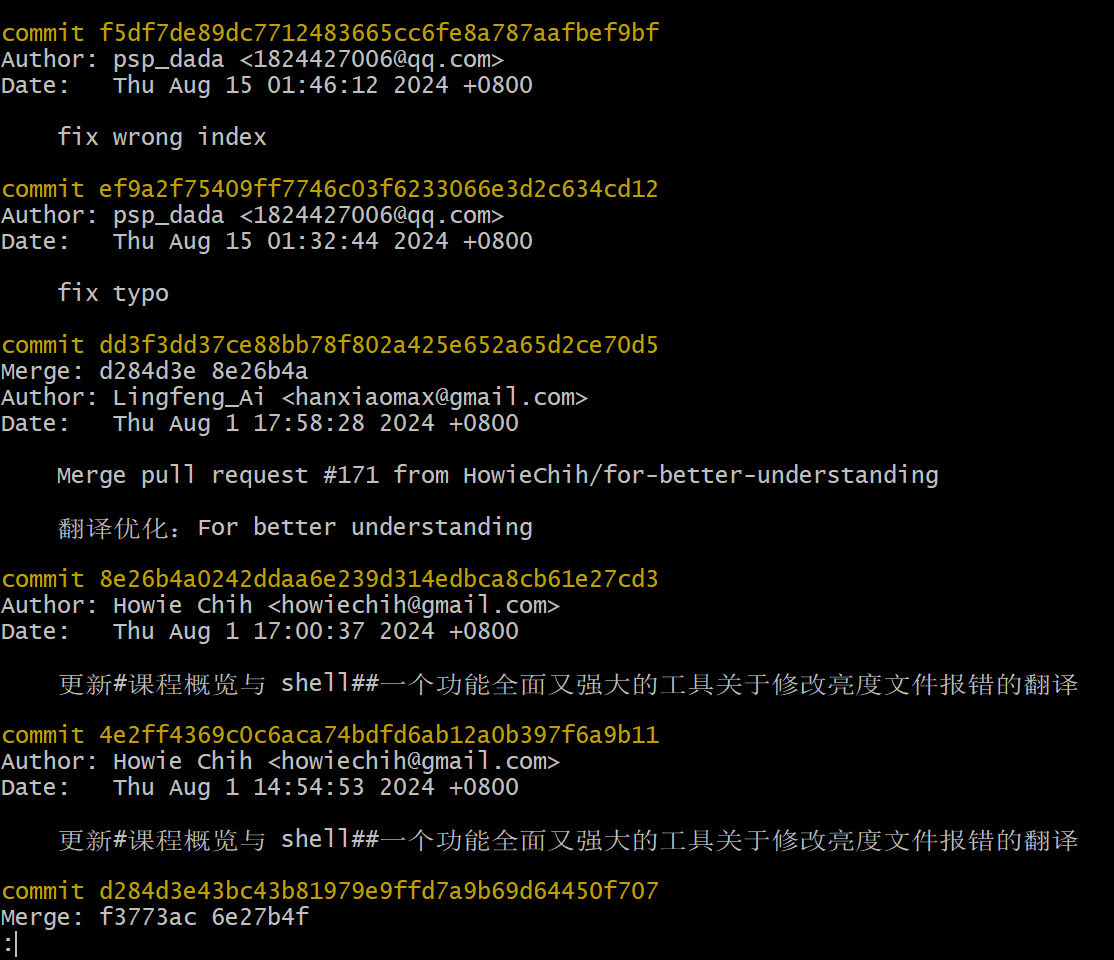
\includegraphics[width = 16cm]{8}
	
	然后,我们再来清除提交记录,在Git中依次输入git filter-branch --force --index-filter\ 、 'git rm --cached --ignore-unmatch ./my\_password' \ 、--prune-empty --tag-name-filter cat -- --all,即可清除。
	
	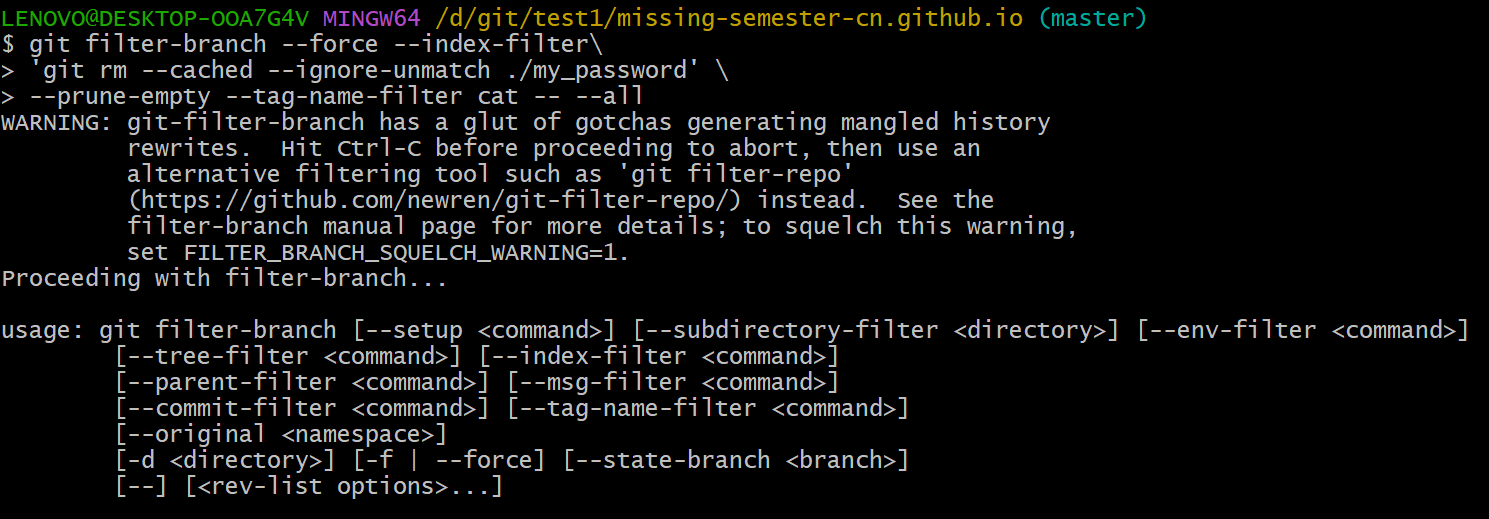
\includegraphics[width = 16cm]{9}
	
	\section{实验中遇到的问题与解决方法}
	\subsection{在进行Github上仓库的克隆时,出现 Git 无法验证 GitHub 的 SSL 证书的报错}
	在搜索报错语句后得知,这是本地的证书问题或网络问题导致的。在Git中输入代码git config --global http.sslVerify false,这样就可以绕过 SSL 证书检查,成功克隆仓库。
	\subsection{在进行课堂练习——向克隆下来的仓库中提交敏感信息时,无法提交,显示who you are?的提示}
	这是因为没有登记个人信息,在命令行终端输入指令git config --global user.email "邮箱"、git config --global user.name "名称",登记个人名称和邮箱之后即可继续进行。
	\subsection{在使用Latex进行文本编辑时,只能用英文进行编辑,使用中文会发生错误}
	在查阅相关书籍后得知,这是因为Texstudio默认用来编辑英文文档,无法识别中文,如果要编写中文文档需要在文档最上面写上代码documentclass[UTF8,a4paper]\{ctexart\},让中文能够被识别,但是涉及到中英文都有的文档编写,就会展现出弊端——英文文本也是以中文的形式显示,具体体现在英文语句中的符号会被转换为中文输入法中的相应符号。
	\subsection{使用Texstudio撰写实验报告时,发现编译出来的PDF文档中出现部分文字无法显示或显示不全的问题}
	这是由于页边距没有调整好,需要在文档中加入geometry拓展包,然后用geometry指令来修改合适的页边距,即可将文本完全显示。
	\subsection{在插入图片时,发现即使加入了graphicx拓展包也无法插入}
	这是因为在中文文本中,想要插入图片需要将图片打包成一个文件夹后,放在与tex文件同一目录中,然后再通过语句graphicspath引入图片所在的文件夹,用includegraphics语句来表示要插入的图片、设置图片的长宽。
	\subsection{完成文本写作后,发现第一页是空白页,文本内容从第二页开始}
	这是应为第一页默认为封面页,需要添加封面。
	
	\section{实例练习}
	\subsection{初始化Git仓库}
	在Git中输入命令git init,即可在当前目录下创建一个新的仓库。
	
	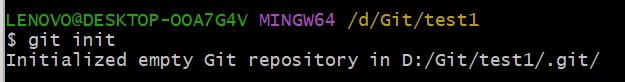
\includegraphics[width = 16cm]{11}
	
	\subsection{查看当前状态}
	输入git status指令,可以显示当前工作目录和暂存区的状态,包括哪些文件被修改了、哪些文件是新添加的等。
	
	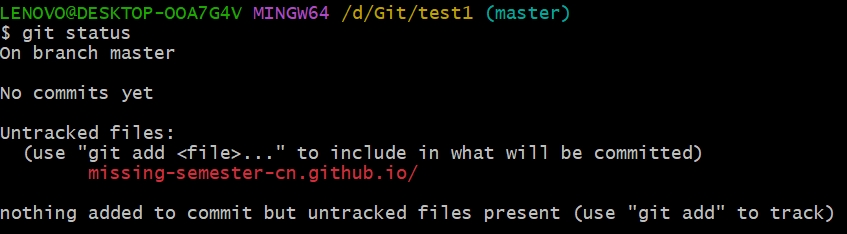
\includegraphics[width = 16cm]{12}
	
	\subsection{添加文件到暂存区}
	git add <文件名>,表示将指定文件添加到暂存区,准备提交。
	
	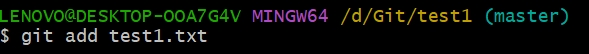
\includegraphics[width = 16cm]{131}
	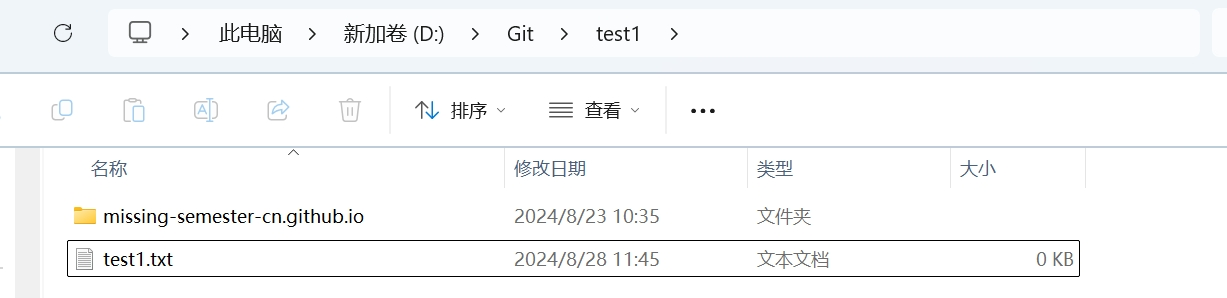
\includegraphics[width = 16cm]{132}
	
	\subsection{提交更改}
	git commit -m "提交信息",将暂存区的更改提交到仓库中,并附上提交信息。
	
	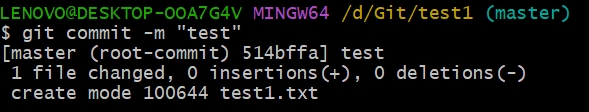
\includegraphics[width = 16cm]{14}
	
	\subsection{查看提交历史}
	git log,显示当前分支的提交历史,包括提交ID、作者、日期和提交信息。
	
	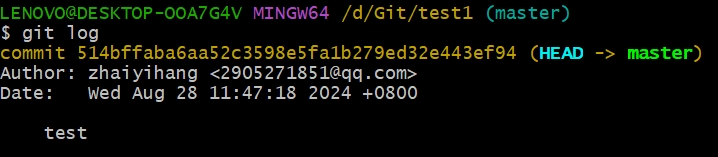
\includegraphics[width = 16cm]{15}
	
	\subsection{查看文件差异}
	git diff,查看工作目录中已修改但尚未暂存的文件与最后一次提交之间的差异。若要查看暂存区与最后一次提交之间的差异,可以使用git diff --cached。
	
	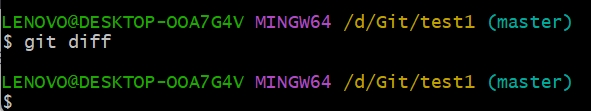
\includegraphics[width = 16cm]{16}
	
	\subsection{撤销工作目录的更改}
	git checkout -- <文件名>,将指定文件从暂存区或最近一次提交中检出到工作目录,以撤销工作目录中的更改。
	
	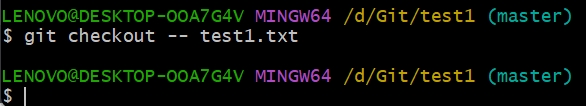
\includegraphics[width = 16cm]{17}
	
	\subsection{撤销暂存区的更改}
	git reset HEAD <文件名>,将指定文件从暂存区撤销,回到工作目录,但文件内容不会改变(仅取消暂存)。
	
	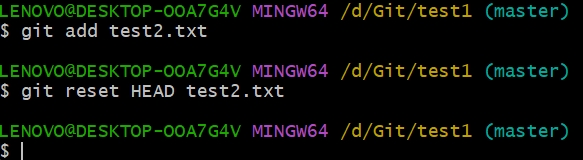
\includegraphics[width = 16cm]{18}
	
	\subsection{切换到其他分支}
	git checkout <分支名>,切换到指定分支。如果分支不存在,则会报错。
	
	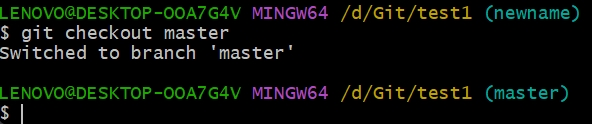
\includegraphics[width = 16cm]{19}
	
	\subsection{创建并切换新分支}
	git checkout -b <新分支名>,创建并切换到一个新的分支。这个命令是git branch <新分支名>和git checkout <新分支名>的合并。
	
	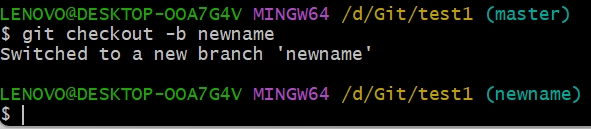
\includegraphics[width = 16cm]{20}
	
	\subsection{查看远程仓库信息}
	git remote -v,这个命令会列出所有配置的远程仓库及其URL。
	
	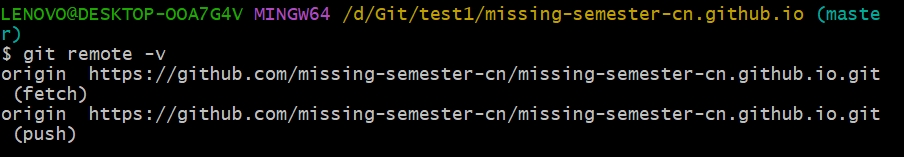
\includegraphics[width = 16cm]{21}
	
	\subsection{克隆远程仓库}
	git~~~clone<仓库URL>,克隆一个远程仓库到本地目录。(由于该实例在课堂练习的准备阶段已经克隆过Github上的一个仓库,在此处不再附加图片展示)
	
	\subsection{删除本地分支}
	git branch -D <分支名>,-D是大写的,用于强制删除分支,即使分支未合并。如果只是想删除已合并的分支,可以使用-d。
	
	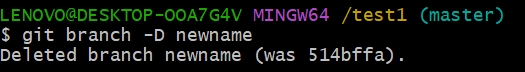
\includegraphics[width = 16cm]{23}
	
	\subsection{比较暂存区与最近一次提交的差异}
	git diff --cached,显示暂存区与最近一次提交之间的差异。
	
	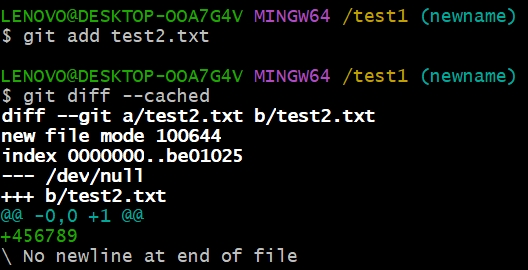
\includegraphics[width = 16cm]{24}
	
	\subsection{合并分支}
	git checkout <目标分支> 、git merge <源分支>,将<源分支>的更改合并到<目标分支>中。
	
	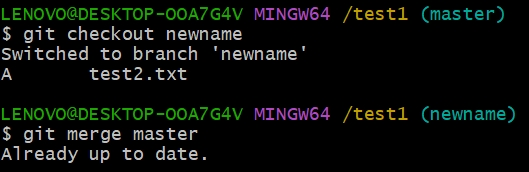
\includegraphics[width = 16cm]{25}
	
	\subsection{查看分支列表}
	
	git branch,列出本地分支。
	
	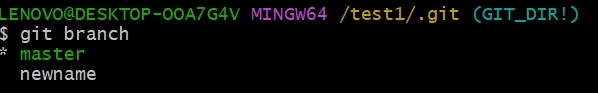
\includegraphics[width = 16cm]{26}
	
	\subsection{用Latex创建一个简单的文档}
	
	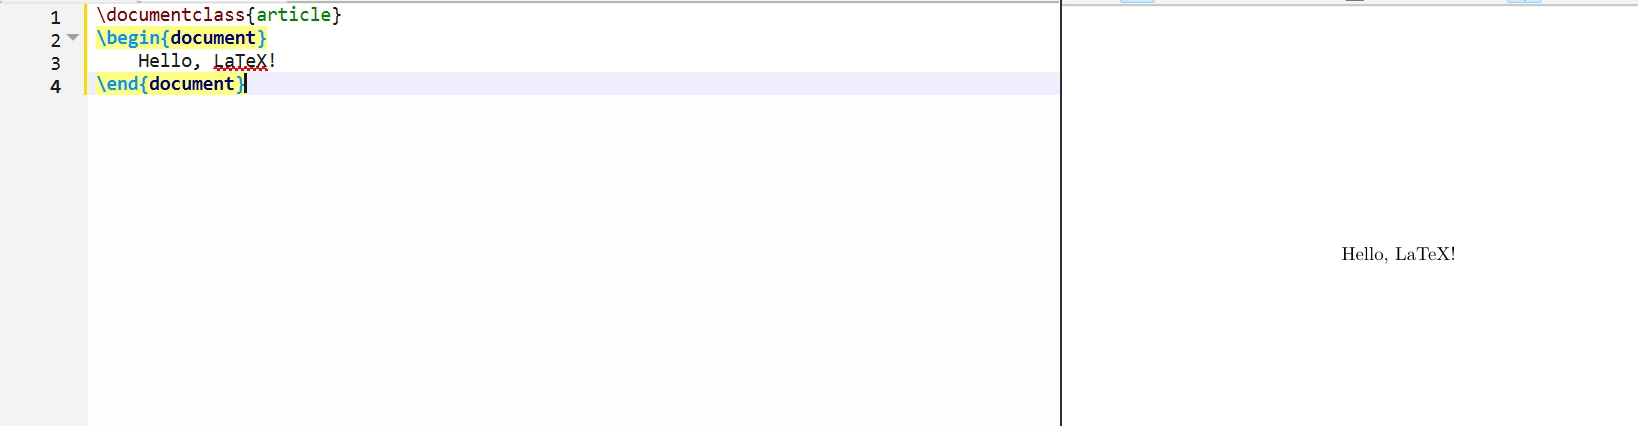
\includegraphics[width = 16cm]{27}
	
	\subsection{添加标题和作者}
	
	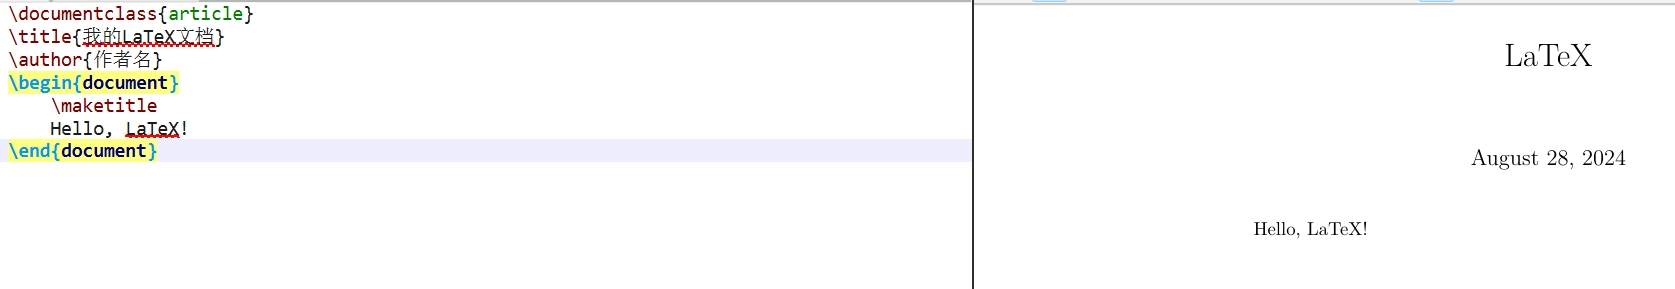
\includegraphics[width = 16cm]{28}
	
	\subsection{插入数学公式}
	
	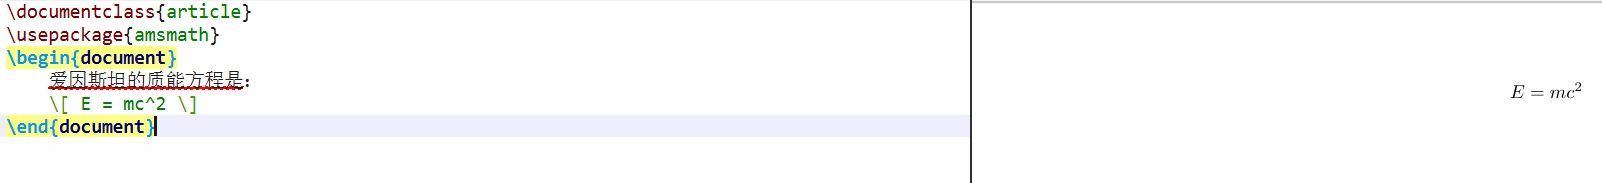
\includegraphics[width = 16cm]{29}	
	
	\subsection{注释}
	% 这是一个注释,不会出现在最终的文档中。
	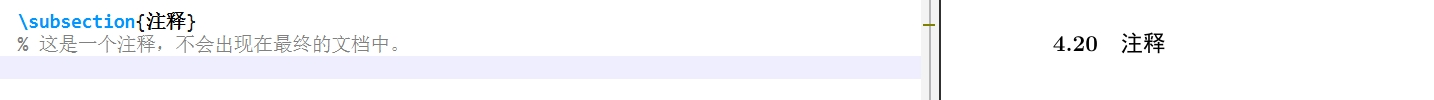
\includegraphics[width = 16cm]{30}	
	
	\section{实验收获与感悟}
	通过学习Git与Latex,我深刻认识到了版本控制在项目管理中的重要性,也知道Git可以对有效记录进行更改、解决冲突;掌握了掌握Git分支与合并技巧,同时也明白Git可以成为团队协作的桥梁,用来减少沟通成本,提升效率;此次对于Git的学习也使我进一步适应了其独特的工作和思维方式。LaTeX拥有卓越的排版能力,可以生成生成美观、专业的文档;同时,其强大的数学公式编辑功能,可以轻松呈现复杂数学表达式,提升论文可读性,并使之符合学术规范;除此之外我可以在网上查找合适、美观的论文模板,并将其tex文件直接移植过来方便自己应用,大大提高了写论文的工作效率,这为我将来撰写数学建模比赛论文打下了坚实的基础。
	
	学习Git和LaTeX的过程虽然充满挑战,但它们带给我的收获和感悟却是无法估量的。Git让我掌握了版本控制和团队协作的精髓,而LaTeX则让我能够以更加专业和高效的方式编写文档。这两种工具不仅提升了我的技术能力,还让我更加深入地理解了项目管理和学术研究的本质。我相信在未来的学习和工作中,它们将继续发挥重要作用并助我一臂之力。
	
	Github仓库链接:https://github.com/Locusclaer/-.git
	
\end{sloppypar}
\end{document}